\documentclass{report}
%\usepackage[margin=5mm,a5paper]{geometry}

%Packages, die für die deutsch Sprache erforderlich sind
\usepackage[utf8]{inputenc}
\usepackage[T1]{fontenc}
\usepackage{lmodern}
\usepackage{ngerman}

%Packages für Graphik
\usepackage{graphicx}
\graphicspath{{Abbildungen/}}

%Optionen für Grafik
% Define new length
\newlength{\myFigureStandardWidth}
% Set the new length to a specific value
\setlength{\myFigureStandardWidth}{1.0\textwidth}

%Package, damit Bibtex-URL klappt
\usepackage{url}

%Package für schöne Tabellen mit variabler Breite
\usepackage{tabularx}
\usepackage{booktabs}
\usepackage{multirow}

%Noch schönere Typographie (gibts nicht in Latexml)
%\usepackage{microtype}

%Pfeile für Chemische Formeln
\usepackage{amssymb}

%Package für Hyperlinks im PDF
\usepackage{hyperref}

%Float-Placement
\usepackage{placeins}

\begin{document}
%%%%% BEGINN TITELSEITE %%%%%

%%%%% ENDE TITELSEITE %%%%%
\chapter*{Abstract}
\addcontentsline{toc}{chapter}{Abstract}
\section*{English}
\selectlanguage{english}
Using a simulation model the technical characteristics of different combinations of charging systems and energy storage systems (= batteries) were computed for two different bus routes. Input data for the simulation were the mechanical and electrical parameters of the charging systems and of the batteries, the mechanical parameters of the bus as well as a recording of a regular passenger transport trip on the respective bus route. For each combination of charging system and energy storage system, the simulation computed the smallest battery required to operate this bus route under defined conditions (e.g. overnight charging versus opportunity charging). For every combination, the output parameters battery size, energy consumption, battery cooling requirement and charging time were calculated.

Based on the simulation results subsequently a weighted assessment was carried out according to VDI 2225 to compare the technical suitability of each combination. Significant differences were observed in the suitability of different combinations of technologies.

Using the methods developed in this study, transportation agencies and policy makers can obtain reliable data on the technical characteristics of different battery-powered buses in order to make a well-informed decision for a specific combination of technologies for charging and for energy storage.


\section*{Deutsch}
\selectlanguage{ngerman}
Mit Hilfe eines Simulationsmodells werden technische Charakteristika von verschiedenen Kombinationen von Ladesystem und Speichertechnologien für zwei unterschiedliche Streckenführungen (Buslinien) berechnet. Eingangsdaten der Simulation sind mechanische und elektrische Parameter von verschiedenen Ladesystemen und Speichertechnologien, die mechanischen Parameter des Busses sowie die Aufzeichnung einer Linienverkehrs-Fahrt auf der jeweiligen Buslinie. Die Simulation berechnet für jede Kombination von Ladesystem und Speichertechnologie die kleinste Batterie, mit der diese Buslinie unter definierbaren Randbedingungen (z.B. Gelegenheits- oder Nachtladung) gefahren werden kann. Für jede Kombination werden Batteriegröße, Energieverbrauch, Batteriekühlung und Ladezeit berechnet.

Auf Basis der Simulationsergebnisse wird anschließend eine Bewertung nach VDI2225 durchgeführt, um die technische Eignung der verschiedenen Kombinationen zu vergleichen. Es zeigen sich deutliche Unterschiede in der Eignung verschiedener Technologiekombinationen.

Mit der in dieser Arbeit vorgestellten Methode können Verkehrsbetriebe sowie politische und wirtschaftliche Entscheidungsträger zuverlässige Daten über die technischen Charakteristika von verschiedenen batteriebetriebenen Bussen erhalten und auf dieser Grundlage eine fundierte Entscheidung für eine bestimmte Technologiekombination treffen.
\chapter*{Aufgabenstellung}
\addcontentsline{toc}{chapter}{Aufgabenstellung}

\section*{Problemstellung und Zielsetzung}
Zwei der wichtigsten Fragen beim Einsatz von batteriebetriebenen Stadtbussen sind, wie der Bus aufgeladen wird und wie die Energie im Bus gespeichert wird. Inzwischen sind diverse Ladesysteme weit genug entwickelt, um im praktischen Betrieb eingesetzt zu werden. Praktisch einsetzbare Speichertechnologien existieren bereits und laufend werden neue Forschungsergebnisse im Bereich der Batterietechnologien schnell industriell umgesetzt.

In dieser Bachelorarbeit werden verschiedene Ladesysteme und Speichertechnologien verglichen. Die Systeme werden hierbei aus technischer Sicht betrachtet, zum Beispiel unter Berücksichtigung mechanischer, elektrischer und sicherheitstechnischer Parameter. Wirtschaftliche und politische Aspekte werden nicht explizit untersucht. Es werden Ladesysteme verglichen, die bereits im normalen Verkehrsbetrieb erprobt wurden oder werden. Bei den Speichertechnologien werden nur Technologien verglichen, die jetzt oder in naher Zukunft im industriellen Maßstab produziert werden können.

Ziel ist es, die Effizienz verschiedener Kombinationen von Ladetechnologie, Speichertechnologie und Ladestrategie auf verschiedenen Buslinien vergleichen zu können.

\section*{Grundsätzliche Vorgehensweise}
\begin{enumerate}
	\item Überblick über existierende Ladesysteme und Speichertechnologien für Elektrobusse
	\item systematische Festlegung der technischen Parameter, nach denen die Eignung der verschiedenen Ladesysteme und Speichertechnologien beurteilt wird
	\item Modellrechnungen zur Ermittlung der für jede Kombination von Ladesystem und Speichertechnologie unterschiedlichen Werte
	\item Ermittlung der besten Technologiekombination für zwei ausgesuchte Strecken und Diskussion der Ergebnisse
\end{enumerate}

\tableofcontents
\newpage

%%%%% BEGINN INHALT %%%%%
\pagenumbering{arabic}

\chapter{Einleitung}
\section{Kontext} %Namen ändern!
\subsection{Geschichte}
\subsection{Aktueller Stand}
\section{Problem} %TODO Namen ändern
\subsection{Ziel} %TODO: Nur im Text erwähnen?
\section{Methodik} %(Kurz))
\chapter{Ladesysteme} %Zewitens
\section{Bewertungskriterien} %TODO: Subsections
% Mit welcher Methode ausgewählt?
\section{Betrachtete Systeme} %TODO: Subsections
\section{Vergleichstabelle}
\chapter{Speichertechnologien} %Zuerst
Nach den Ladesystemen werden in diesem Kapitel nun die Energiespeicher für Stadtbusse betrachtet. Wie im vorigen Kapitel werden zunächst die Bewertungskriterien und die betrachteten Technologien erläutert. In Tabelle \ref{vergleichstabelle_speichertechnologien} auf Seite \pageref{vergleichstabelle_speichertechnologien} werden die Werte aufgelistet.\\
Im Gegensatz zu den Ladesystemen ist die Produktvielfalt der Speichertechnologien nahezu unbegrenzt. Von daher werden hier keine konkreten Produkte verglichen, sondern es wurde versucht, die jeweils für den aktuellen Stand der Speichertechnologie relevanten Kenndaten zu finden.
\section{Bewertungskriterien} %TODO: Subsections
\section{Betrachtete Technologien}
Im folgenden Abschnitt werden die Grundlagen und die Einsatzgeschichten der verschiedenen Speichertechnologien kurz erläutert. Die Technologien sind nach dem genutzten physikalischen Effekt aufgeteilt \cite{Sterner:2014}[S. 35f].
\subsection{Mechanisch – Schwungradspeicher} %TODO: Quellen, warum endete die Gyrobuserprobung
In Bussen kann mechanische Energie mit einem Schwungrad gespeichert werden\footnote{Es gibt auch Prototypen von Pressluftspeichern in kleineren Fahrzeugen, in Bussen werden sie jedoch nur als Teil eines Hybridantriebs eingesetzt und hier nicht weiter betrachtet \cite{Sebastian-Naumann:2014}[S. 14].}, das die elektrische Energie in der Rotation des Schwungrades speichert. Die Energieübertragung erfolgt durch eine elektrische Motor- und Generatoreinheit. Moderne Schwungräder werden aus gewickelten Karbonfasern hergestellt und in Vakuumgehäusen magnetisch gelagert, sie erreichen hohe Drehzahlen und geringe Reibungsverluste \cite{993788}. Im Falle eines berstenden Schwungrades muss das Gehäuse die gesamte Energie innerhalb von Sekundenbruchteilen aufnehmen, ohne selbst zu bersten. Dies erfordert sehr schwere Gehäuse, die die spezifische Energie und Leistung eines tatsächlichen Systems stark reduzieren. Der Schwungradspeicher wurde in den fünfziger Jahren im Gyrobus im schweizerischen Yverdon auf einer acht Kilometer langen Linie erprobt. Die Strecke wurde erfolgreich zurückgelegt, die damalige Technologie war jedoch sehr wartungsaufwändig. Aktuell wird der Schwungradspeicher nur als Teil eines hybriden Antriebsstrangs eingesetzt.
\subsection{Elektrisch – Kondensator} %TODO: Quellen
Der Kondensator ist ein rein elektrischer Energiespeicher. Im klassischen Plattenkondensator werden zwei durch einen festes Dielektrikum getrennte Platten elektrisch aufgeladen, die Ladung kann später in Strom umgewandelt werden. Kondensatoren haben eine hohe spezifische Leistung, aber eine sehr geringe spezifische Energie. In Bussen werden sogenannte Superkondensatoren verwendet, die statt eines festen Dielektrikums ein Elektrolyt (meist eine Salz-Wasser-Lösung) verwenden. Die gelösten Ionen werden von der geladenen Platte angezogen, können sie jedoch aufgrund der umgebenden Ionenschicht nicht erreichen. Da der Abstand zwischen Platte un Ionen extrem klein ist, entsteht eine sehr hohe elektrische Kapazität. Eine weitere Kapazitätssteigerung wird durch die Einlagerung von einigen Elektronen des Elektrolyts in den Leiterplatten erreicht (siehe Abb. \ref{abb_doppelschicht}). \cite{Sterner:2014}[S. 167f]\\
\begin{figure}\centering
	 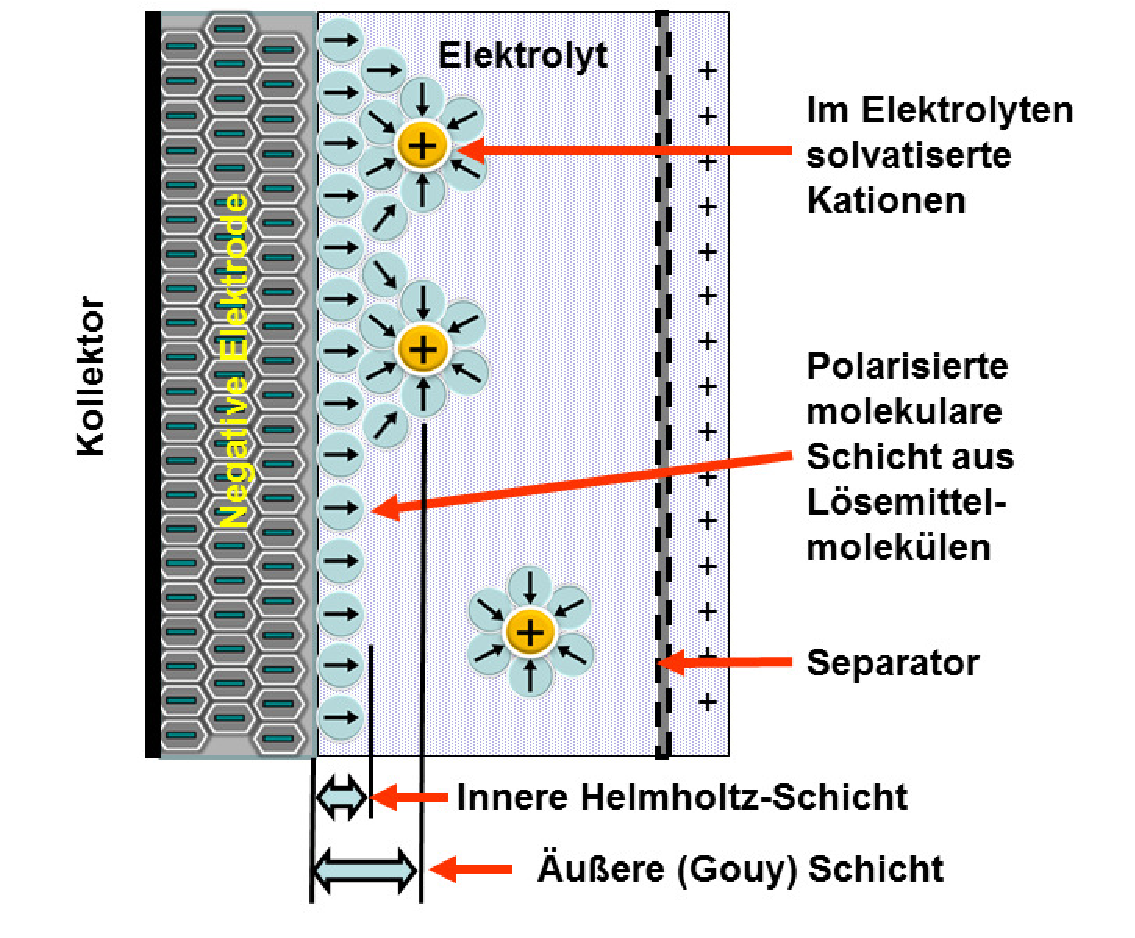
\includegraphics[width=0.5\textwidth]{Doppelschicht-Prinzipdarstellung}
	 \caption{Prinzipdarstellung der Doppelschichtkapazität. Quelle: Elcap (Own work) CC BY-SA 3.0, via Wikimedia Commons}
	 \label{abb_doppelschicht}
\end{figure}
In Shanghai werden Busse mit dieser Technologie seit 2008 im Linienverkehr eingesetzt, daneben werden Superkondensatoren für kurzzeitige Einsätze mit hohem Leistungsbedarf, zum Beispiel zur Bremsenergierückgewinnung oder zur Überbrückung stromloser Stellen in Trolleybussen eingesetzt \cite{Barminer-Busgesellschaft:2012}.
\subsection{Chemisch – Batterie}
\section{Vergleichstabelle}   %TODO: AUSFÜLLEN!
\begin{table}[htbp]\centering
	\begin{tabularx}{\linewidth}{XXX}
		\toprule
		A1 & B1 & C1 \\ \midrule
		A2 & B2 & C2 \\
		A3 & B3 & C3 \\ \bottomrule
	\end{tabularx}
	\caption{Übersicht Ladesysteme}
	\label{vergleichstabelle_speichertechnologien}
\end{table}
\chapter{Effizienzberechnung} %TODO: Besserer Titel %Drittens
\section{Ladesystem}
\section{Speichertechnologie}
\section{Ladestrategie und Route}
\section{Ergebnisse}
\subsection{Route A}
\subsection{Route B}
\chapter{Bewertung und Diskussion} %Diksussion
\section{Fazit}
\section{Ausblick}

%%%%% ENDE INHALT %%%%%

%Bibliographie
\bibliographystyle{alphadin}
\bibliography{../Quellen/Quellenliste} 

\appendix
\label{an_Datenblaetter}
\chapter{Datenblätter}
\begin{figure}[h!]\centering
	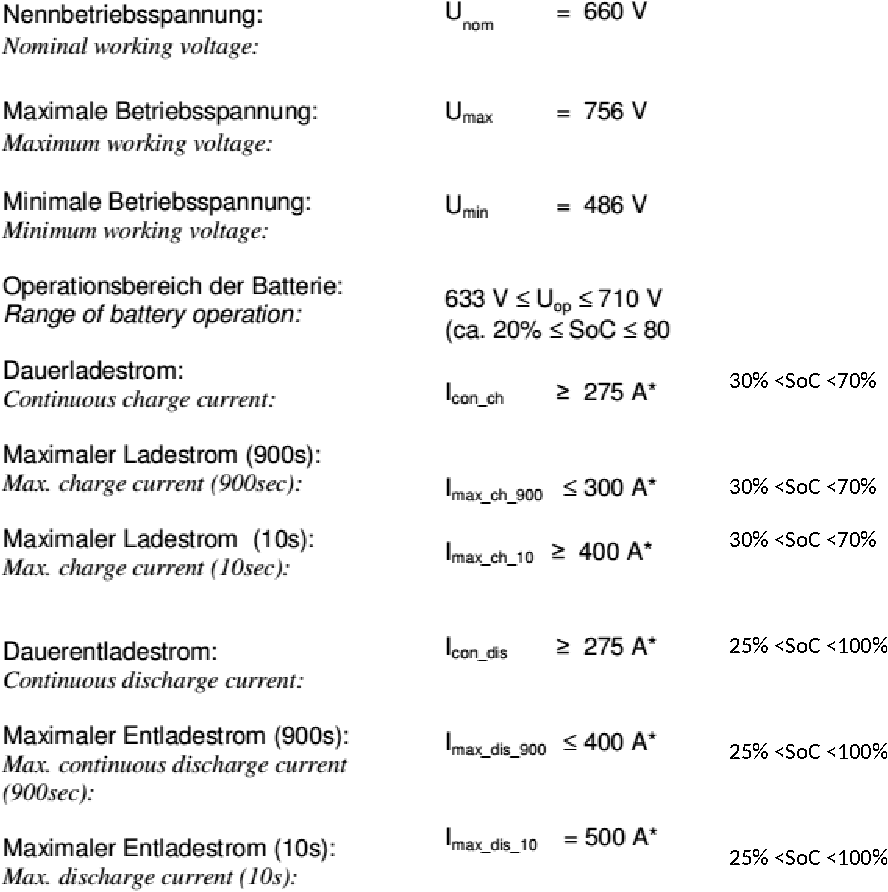
\includegraphics[height=15.5cm]{Datenblatt_LTO}
	\caption[Daten zum Primove-Akku]{Daten zum Primove-Akku. Quelle: MPM TU Berlin}
\end{figure}

\begin{figure}\centering
	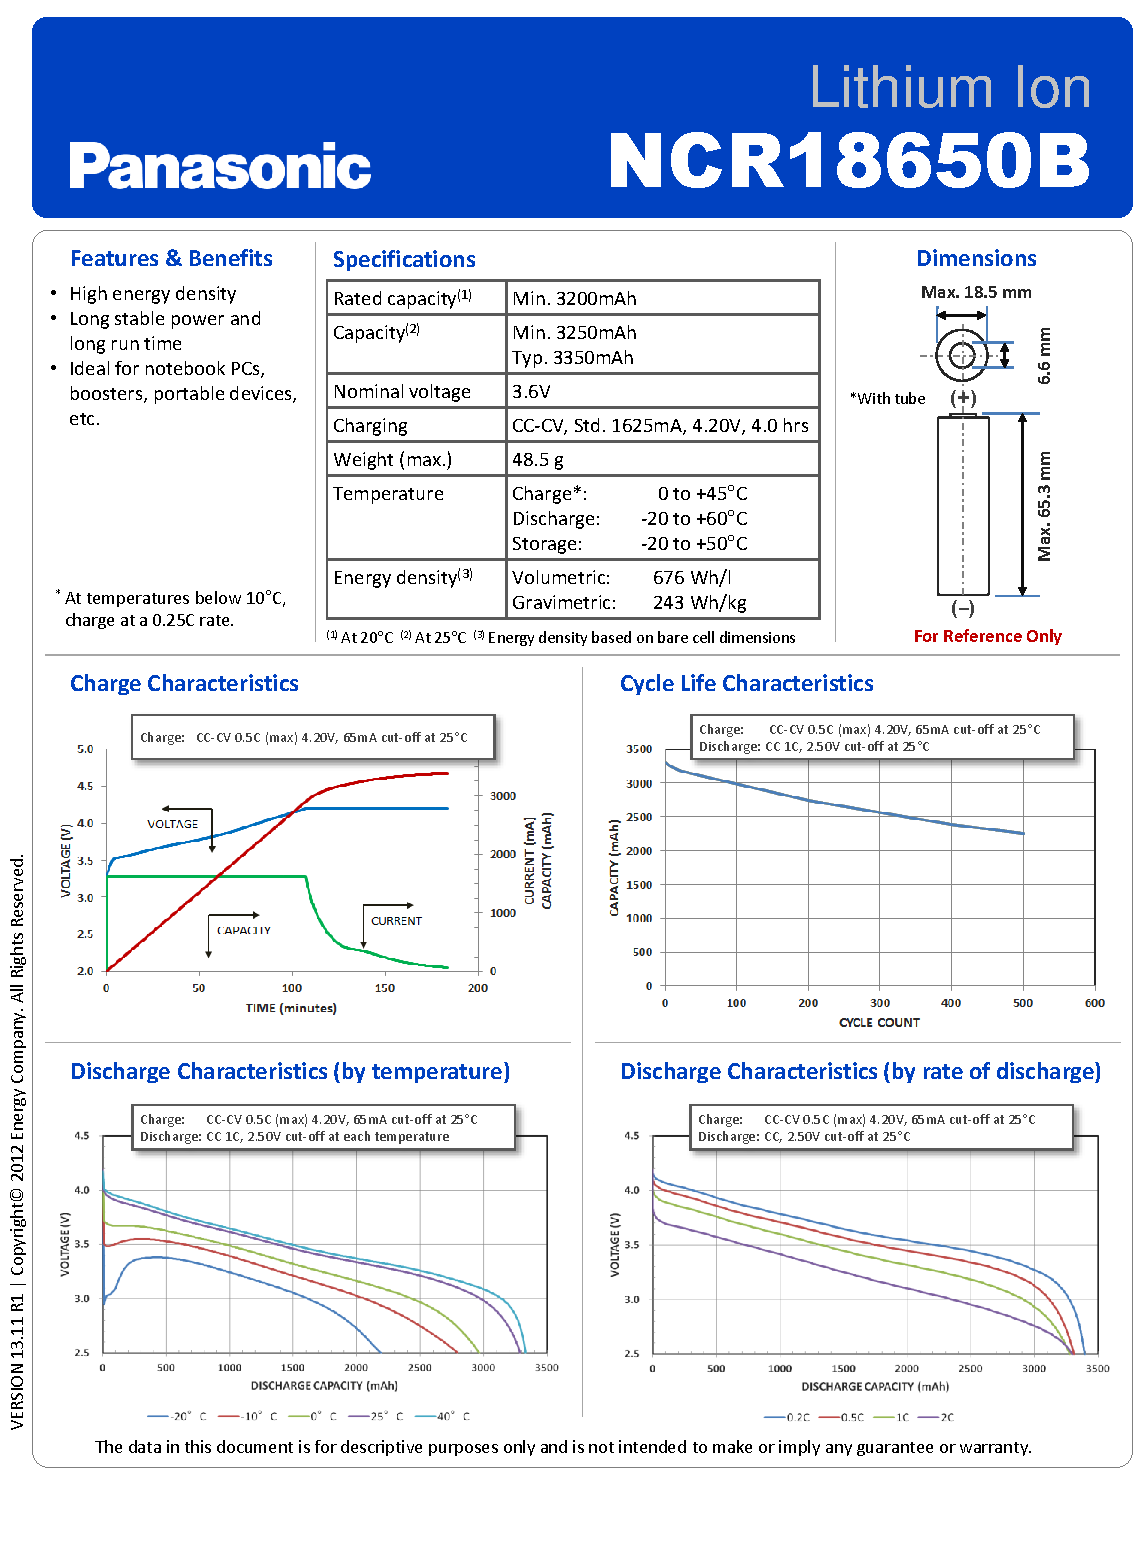
\includegraphics[height=20cm]{Datenblatt_18650}
	\caption[Datenblatt Panasonic NCR18650B]{Datenblatt Panasonic NCR18650B. Quelle: Panasonic Industrial North America}
\end{figure}

\begin{figure}\centering
	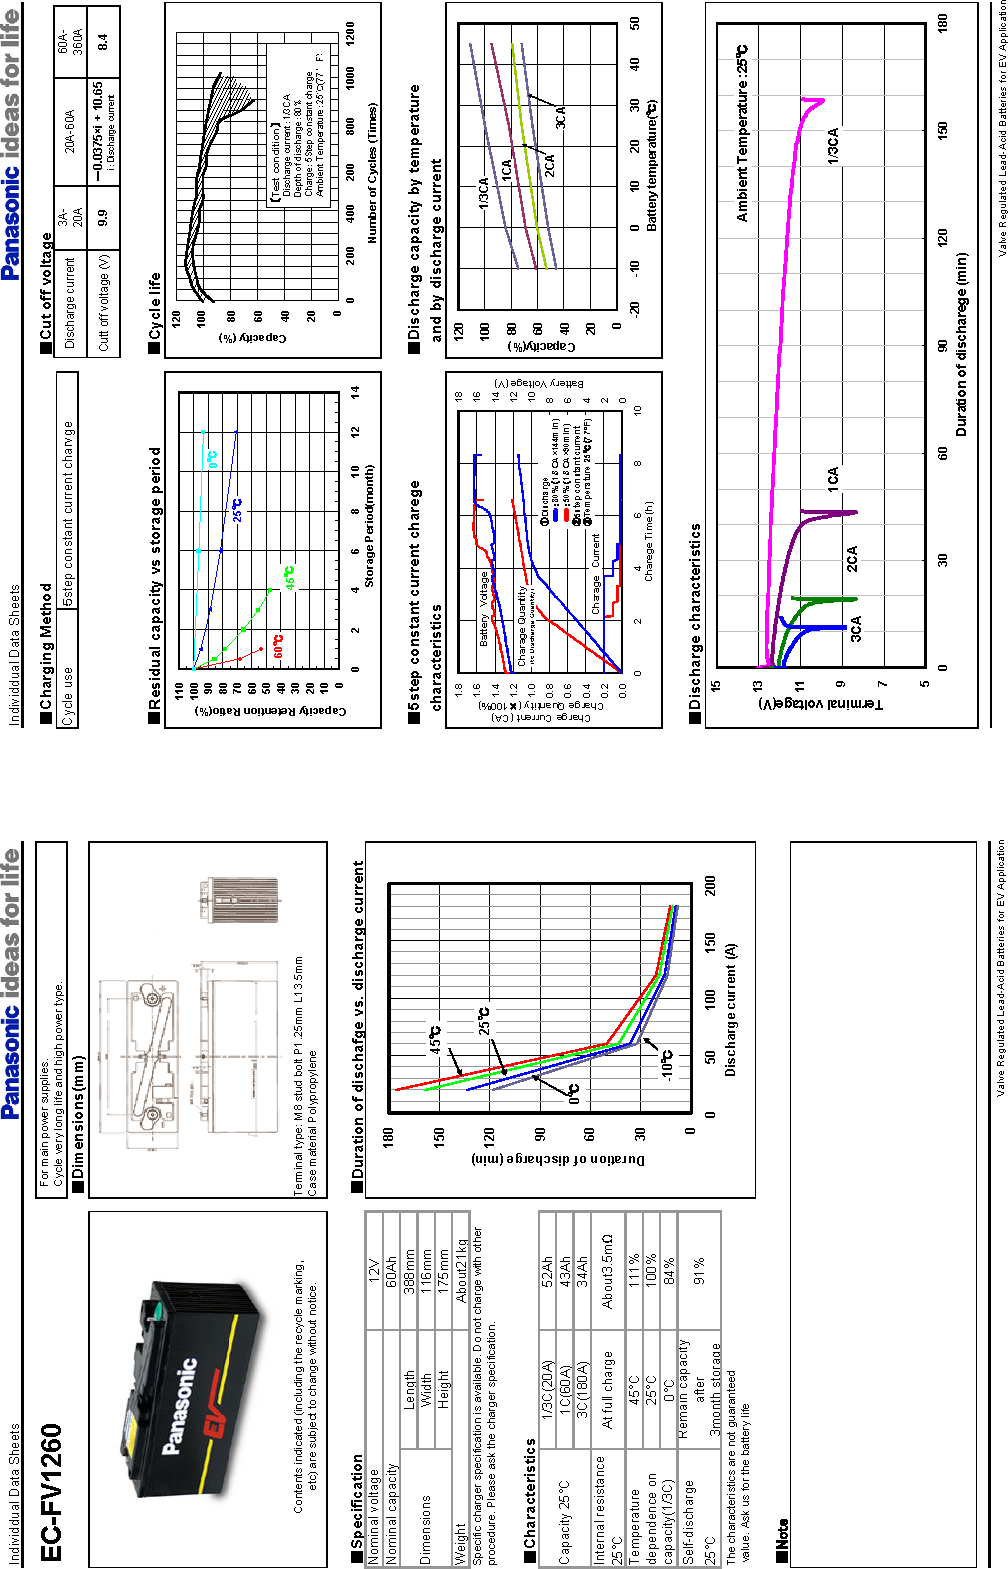
\includegraphics[height=20cm]{Datenblatt_VRLA}
	\caption[Datenblatt Panasonic EC-FV1260]{Datenblatt Panasonic EC-FV1260. Quelle: Panasonic Industrial North America}
\end{figure}

\begin{figure}\centering
	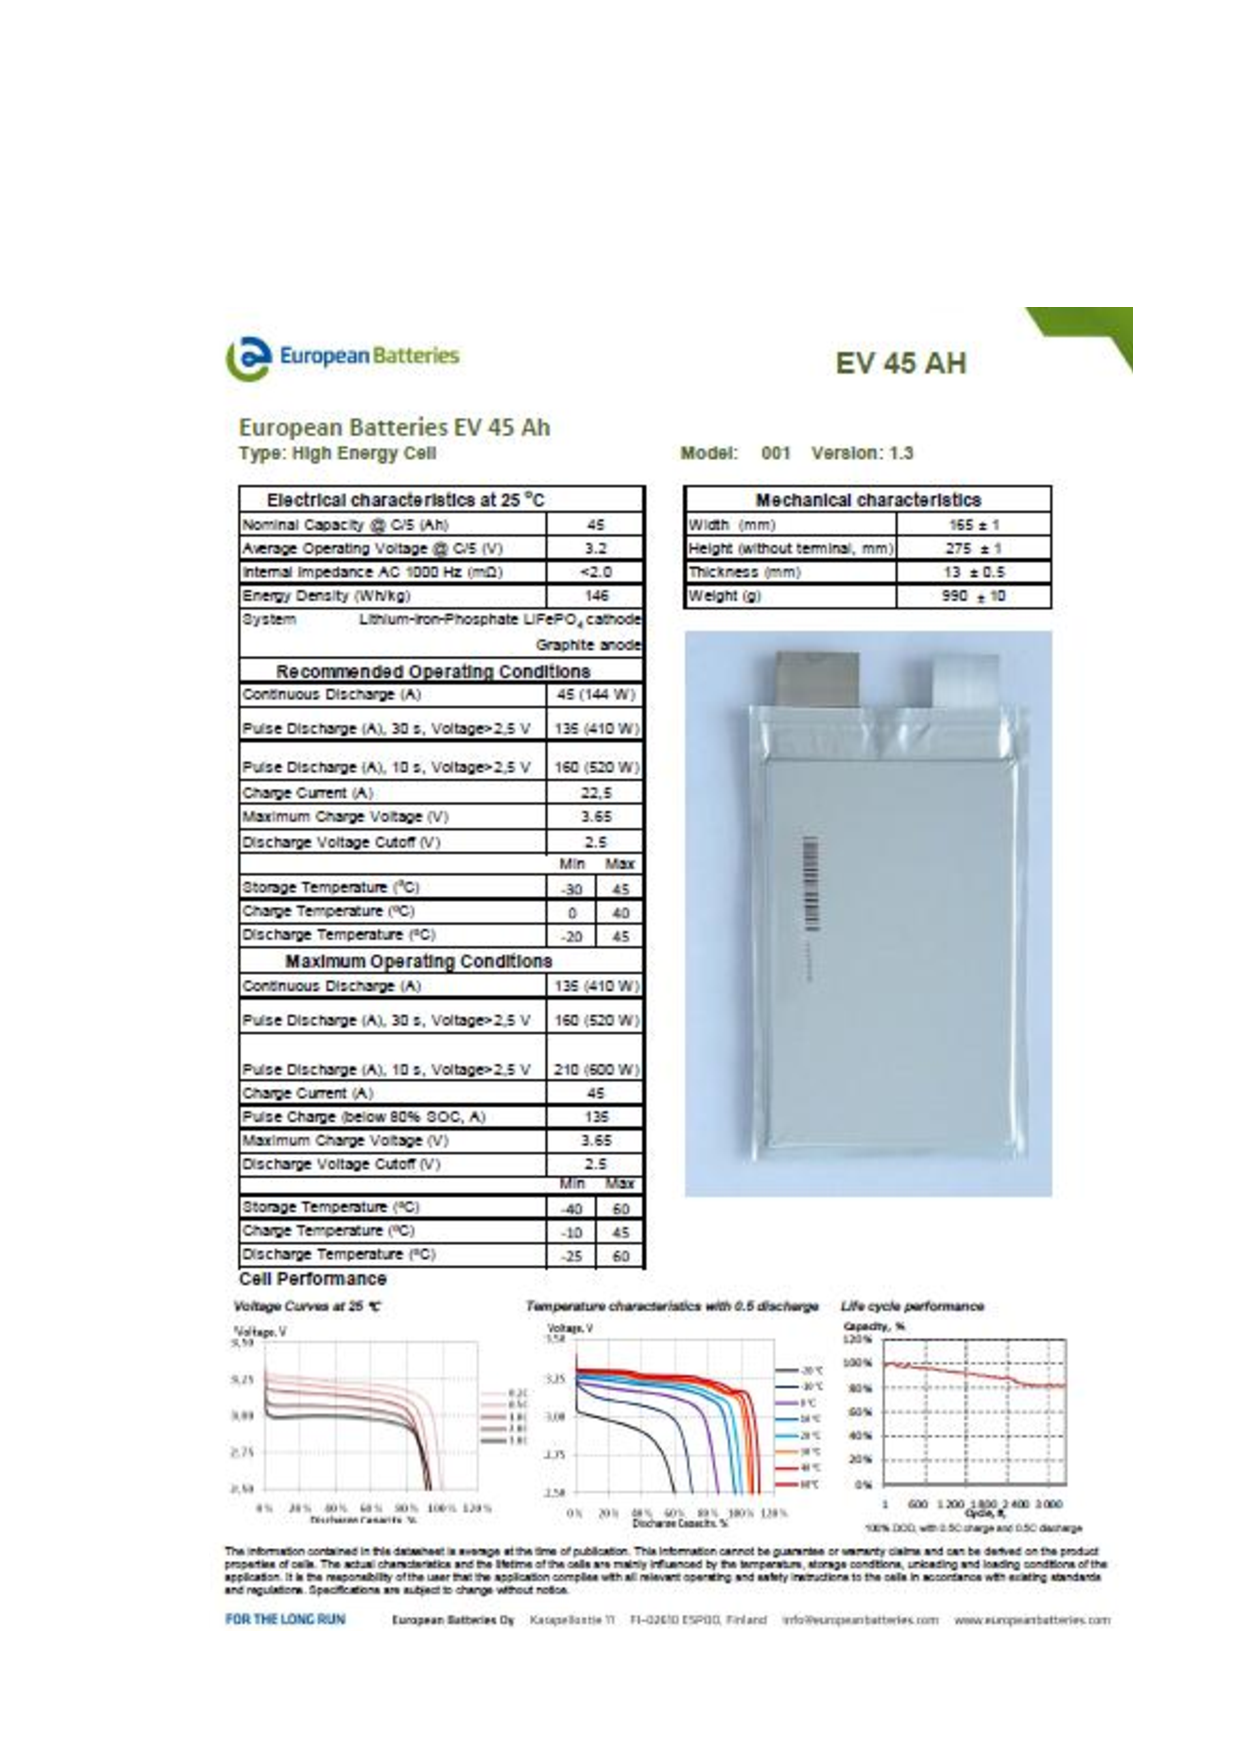
\includegraphics[height=20cm]{Datenblatt_LFP}
	\caption[Datenblatt European Batteries LiFePO EV 45 Ah]{Datenblatt European Batteries LiFePO EV 45 AH. Quelle: SuperLIB Deliverable 4.1 – Cell Specification with Cell Data}
\end{figure}

\begin{figure}\centering
	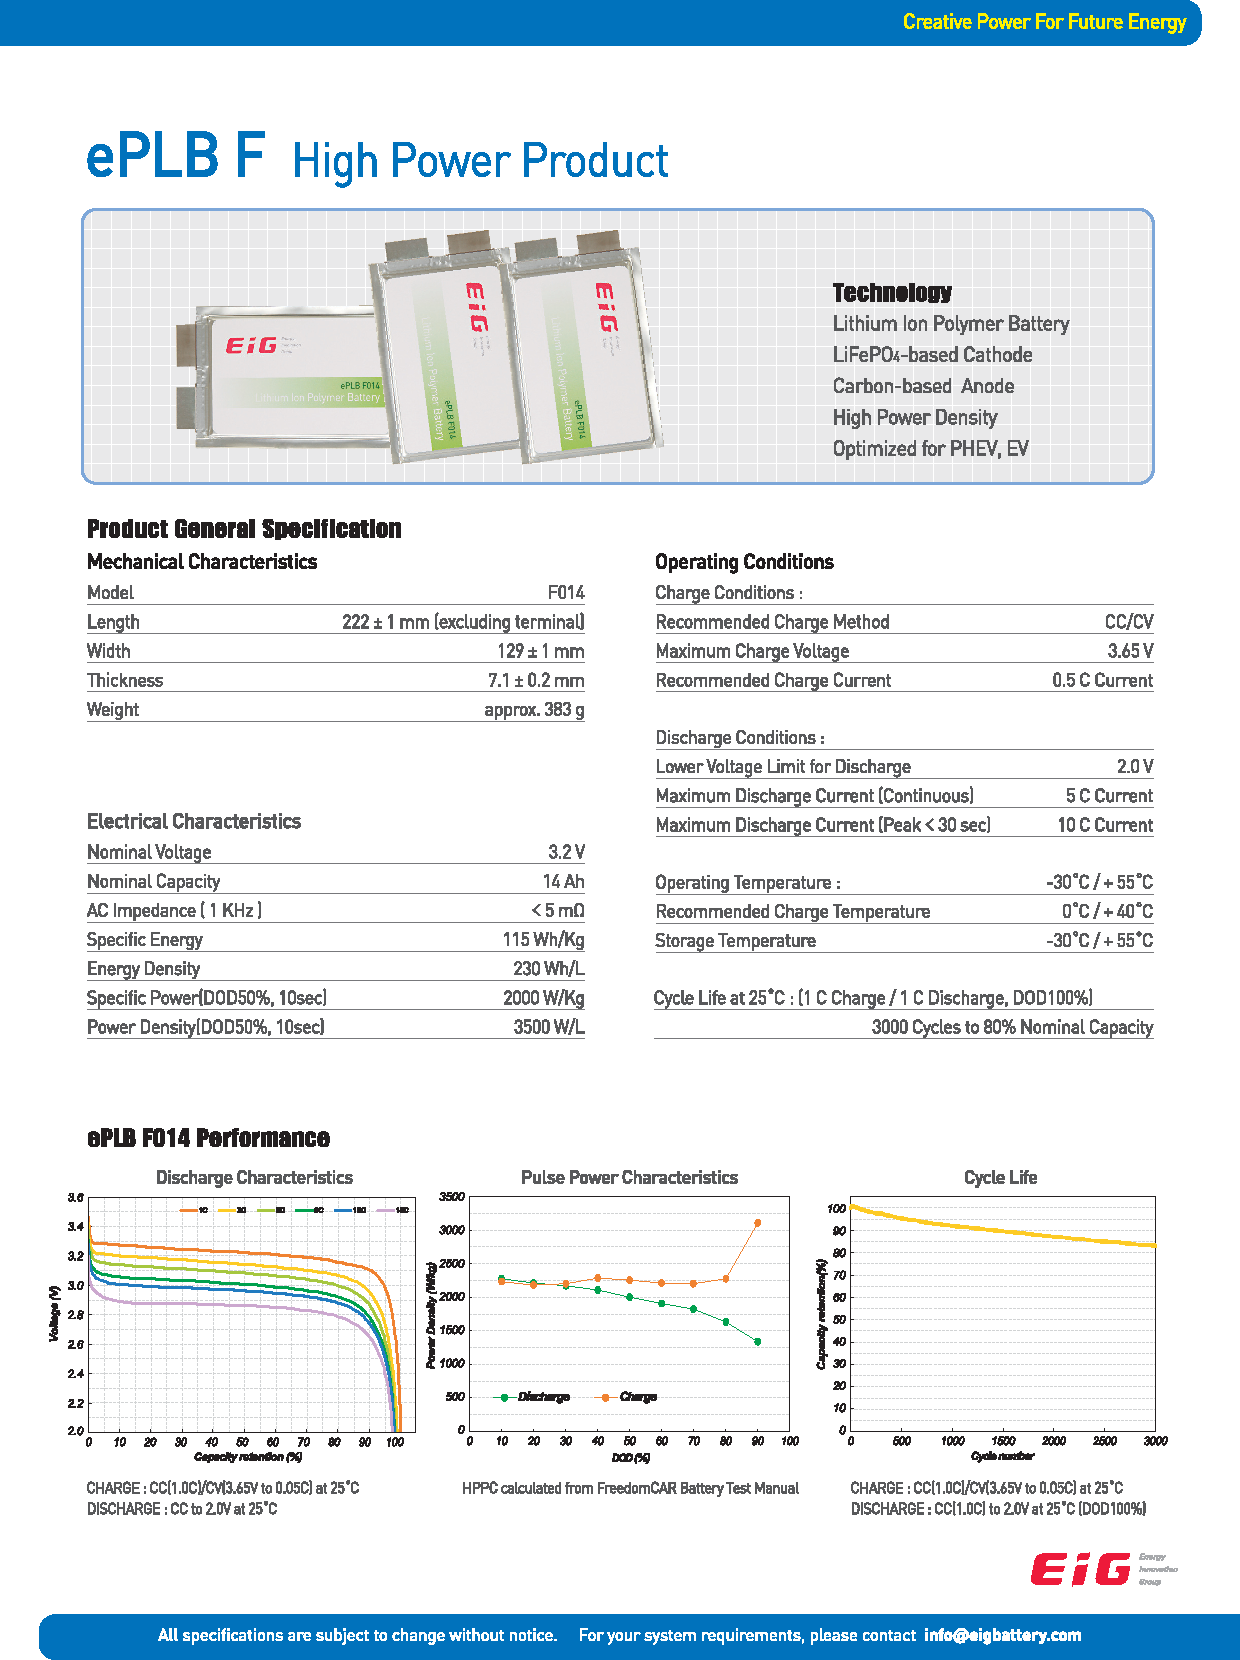
\includegraphics[height=20cm]{Datenblatt_LFP_HP}
	\caption[Datenblatt EIG ePLB F 14 Ah]{Datenblatt EIG ePLB F 14Ah. Quelle: SuperLIB Deliverable 4.1 – Cell Specification with Cell Data}
\end{figure}

\listoffigures
\listoftables

\end{document}
